\documentclass[12pt, letterpaper]{article}
\usepackage[utf8]{inputenc}
\title{Test}
\author{Jeff Mathieu \thanks{niet ik}}
\date{24 april}
\usepackage{graphicx}
\usepackage{parskip}
\graphicspath{{images/}}


\begin{document}
\maketitle
\tableofcontents

\section*{yeet yeet}

\addcontentsline{toc}{section}{yeet yeet}
\section{test 1}

test \LaTeX{} document.\newline
    
%this is a comment

some of the greatest \textbf{test}
discoveries in \underline{yeet}
wow such \textbf{\textit{\underline{elle ma}}}\newline
\subsection{wowow}
Some of the greatest \emph{discoveries} 
in science 
were made by accident.


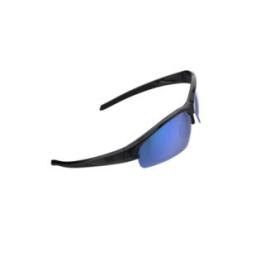
\includegraphics{universe.jpeg}


\begin{enumerate}
    \item The individual entries are indicated with a black dot, a so-called bullet.
    \item The text in the entries may be of any length.
    \item weeeee waarom lijkt dit anders?
\end{enumerate}


\section{test2}
The mass-energy equivalence is described by the famous equation
\[ E=mc^2 \]
discovered in 1905 by Albert Einstein. 
In natural units ($c = 1$), the formula expresses the identity
\begin{equation}
E=m
\end{equation}
\[\frac{e^2}{3} * \frac{1}{3} * \int_0^1 x^2 + 3x + 4dx\]
$\cos(\omega * \alpha)$\newline



Now that we have written our abstract, we can begin writing our first paragraph.
 
This line will start a second Paragraph.

\section{test3}
\subsection{emph}
\textit{Some of the greatest \emph{discoveries} 
in science 
were made by accident.}

\textbf{Some of the greatest \emph{discoveries} 
in science 
were made by accident.}


\subsection{table} 
Table \ref{table:data} is an example of referenced \LaTeX{} elements.
\begin{center}
    

\begin{table}[h!]
\centering
\begin{tabular}{||c c c c||} 
 \hline
 Col1 & Col2 & Col2 & Col3 \\ [0.5ex] 
 \hline\hline
 1 & 6 & 87837 & 787 \\ 
 2 & 7 & 78 & 5415 \\
 3 & 545 & 778 & 7507 \\
 4 & 545 & 18744 & 7560 \\
 5 & 88 & 788 & 6344 \\ [1ex] 
 \hline
\end{tabular}
\caption{Table to test captions and labels}
\label{table:data}
\end{table}

\end{center}

\begin{center}
    \begin{tabular}{|c |c| c|}
        \hline
        [0][0] & [0][0<j<n-1] & [0][n-1]\\
        \hline
        [0<i<n-1][0] & [0<i<n-1][0<j<n-1] & [0<i<n-1][n-1]\\
        \hline
        [n-1][0] & [n-1][0<j<n-1] & [n-1][n-1]\\ 
        \hline
    \end{tabular}
\end{center}

\end{document}